\documentclass[11pt,a4paper,oldfontcommands]{memoir}
\usepackage[utf8]{inputenc}
\usepackage{microtype}
\usepackage[dvips]{graphicx}
\usepackage{xcolor}
\usepackage{times}
\usepackage{graphicx}

\usepackage[
breaklinks=true,colorlinks=true,
%linkcolor=blue,urlcolor=blue,citecolor=blue,% PDF VIEW
linkcolor=black,urlcolor=black,citecolor=black,% PRINT
bookmarks=true,bookmarksopenlevel=2]{hyperref}

\usepackage{geometry}
% PDF VIEW
% \geometry{total={210mm,297mm},
% left=25mm,right=25mm,%
% bindingoffset=0mm, top=25mm,bottom=25mm}
% PRINT
\geometry{total={210mm,297mm},
left=20mm,right=20mm,
bindingoffset=10mm, top=25mm,bottom=25mm}

\OnehalfSpacing
%\linespread{1.3}

%%% CHAPTER'S STYLE
\chapterstyle{bianchi}
%\chapterstyle{ger}
%\chapterstyle{madsen}
%\chapterstyle{ell}
%%% STYLE OF SECTIONS, SUBSECTIONS, AND SUBSUBSECTIONS
\setsecheadstyle{\Large\bfseries\sffamily\raggedright}
\setsubsecheadstyle{\large\bfseries\sffamily\raggedright}
\setsubsubsecheadstyle{\bfseries\sffamily\raggedright}


%%% STYLE OF PAGES NUMBERING
%\pagestyle{companion}\nouppercaseheads 
%\pagestyle{headings}
%\pagestyle{Ruled}
\pagestyle{plain}
\makepagestyle{plain}
\makeevenfoot{plain}{\thepage}{}{}
\makeoddfoot{plain}{}{}{\thepage}
\makeevenhead{plain}{}{}{}
\makeoddhead{plain}{}{}{}


\maxsecnumdepth{subsection} % chapters, sections, and subsections are numbered
\maxtocdepth{subsection} % chapters, sections, and subsections are in the Table of Contents


%%%---%%%---%%%---%%%---%%%---%%%---%%%---%%%---%%%---%%%---%%%---%%%---%%%

\begin{document}

%%%---%%%---%%%---%%%---%%%---%%%---%%%---%%%---%%%---%%%---%%%---%%%---%%%
%   TITLEPAGE
%
%   due to variety of titlepage schemes it is probably better to make titlepage manually
%
%%%---%%%---%%%---%%%---%%%---%%%---%%%---%%%---%%%---%%%---%%%---%%%---%%%
\thispagestyle{empty}

{%%%
\sffamily
\centering
\Large

~\vspace{\fill}

\includegraphics[scale=.5]{marcos.png}
{\huge 
INSTALACIÓN DE ROS EN UBUNTU
}

\vspace{2.5cm}

{\LARGE
Marcos Manzo Torres
}

\vspace{3.5cm}

Universidad Politécnica de la Zona Metropolitana de Guadalajara

\vspace{3.5cm}

Profesor: Carlos Enrique Morán Garabito

\vspace{\fill}

14 de septiembre del 2019

%%%
}%%%

\vspace{1.5cm}




\tableofcontents*

\clearpage

%%%---%%%---%%%---%%%---%%%---%%%---%%%---%%%---%%%---%%%---%%%---%%%---%%%
%%%---%%%---%%%---%%%---%%%---%%%---%%%---%%%---%%%---%%%---%%%---%%%---%%%

\chapter{introducción}

ROS, es un conjunto de bibliotecas de software y herramientas que ayudan a crear aplicaciones roboticas. Desde controladores hasta algoritmos del estado del arte y con potentes herramientas de desarrollo, ROS tiene lo que necesitas para tu próximo proyecto de robótica. 

Entre sus fortalezas está que es usado en investigación, productos comerciales, educación y como centro de entretenimiento, tanto en el sector academico y el sector privado.

En este apartado, aprenderemos a realizar la instalación de ROS en el sistema operativo ubuntu, descargaremos las bibliotecas necesarias para el funcionamiento y creación de campo de trabajo en nuestra computadora.

\section{preparación para instalación}
Primeramente como parte de la instalación, tenemos que configurar nuestro dispositivo para aceptar el software y todos los paquetes de ros.
\begin{figure}[h]
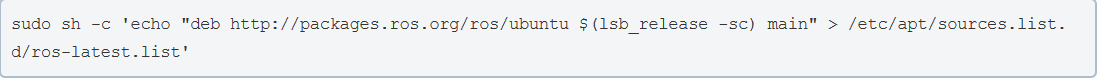
\includegraphics[scale=.8]{link1.png}
\end{figure}

preparamos las llaves de nuestro sistema Ubuntu, como segunda parte del proceso
\begin{figure}[h]
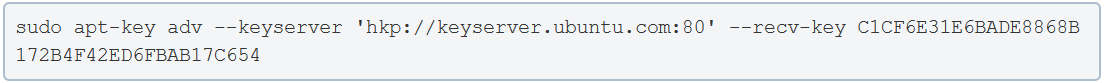
\includegraphics[scale=.8]{link11.png}
\end{figure}

\section{instalación}
procedemos a la instalación de ros, como primer paso nos aseguramos de que nuestro sistema Ubuntu se encuentra actualizado, para ello lanzamos el siguiente código.
\begin{figure}[h]
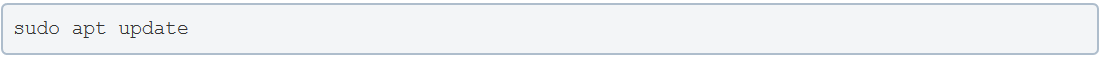
\includegraphics[scale=.8]{link20.png}
\end{figure}
Hay muchas herramientas diferentes en ROS. Se proporciona la configuración básica para que pueda comenzar. 
A continuación tenemos los elementos seleccionados y configuraciones recomendadas
Instalación completa en el escritorio: (recomendado) : ROS, rqt , rviz , bibliotecas genéricas de robots, simuladores 2D / 3D y percepción 2D / 3D

\begin{figure}[h]
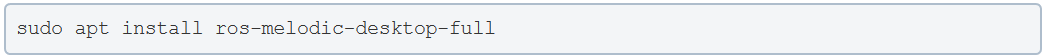
\includegraphics[scale=.8]{link13.png}
\end{figure}

Para encontrar paquetes disponibles después de realizar la instalación, usamos el siguiente código:

\begin{figure}[h]
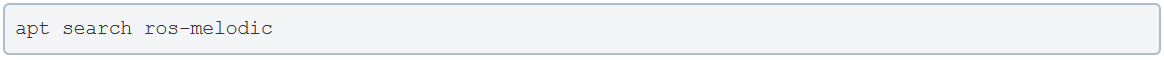
\includegraphics[scale=.8]{link15.png}
\end{figure}

como siguiente paso instalamos rosdep para encontrar fácilmente las dependencias y componentes de ros.

\begin{figure}[h]
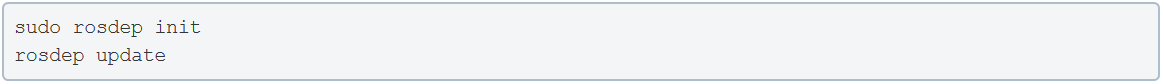
\includegraphics[scale=.8]{link16.png}
\end{figure}

\section{declaración de entorno de trabajo}
Declaramos el archivo setup.bash
Si se tienen varias versiones de ros, se creará un conflicto con el archivo setup.bash, por lo que solo se recomienda una versión y una configuración del archivo setup.bash
después de esto, ya tenemos listo nuestro ambiente de trabajo. la instalación ha finalizado y solo falta realizar la comprobación de la correcta instalación.

\begin{figure}[h]
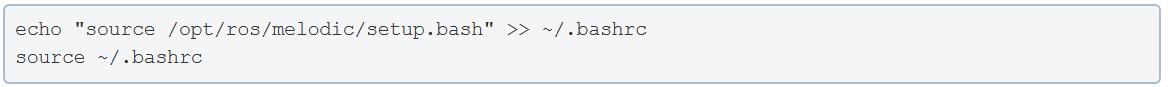
\includegraphics[scale=.8]{link17.png}
\end{figure}


 

\chapter{Comprobación de instalación}
lanzamos el complemento roscore para verificar que la instalación se realizó con exito, nos aparecerá de la siguiente manera (si no se tuvo ningún error)
\begin{figure}[h]
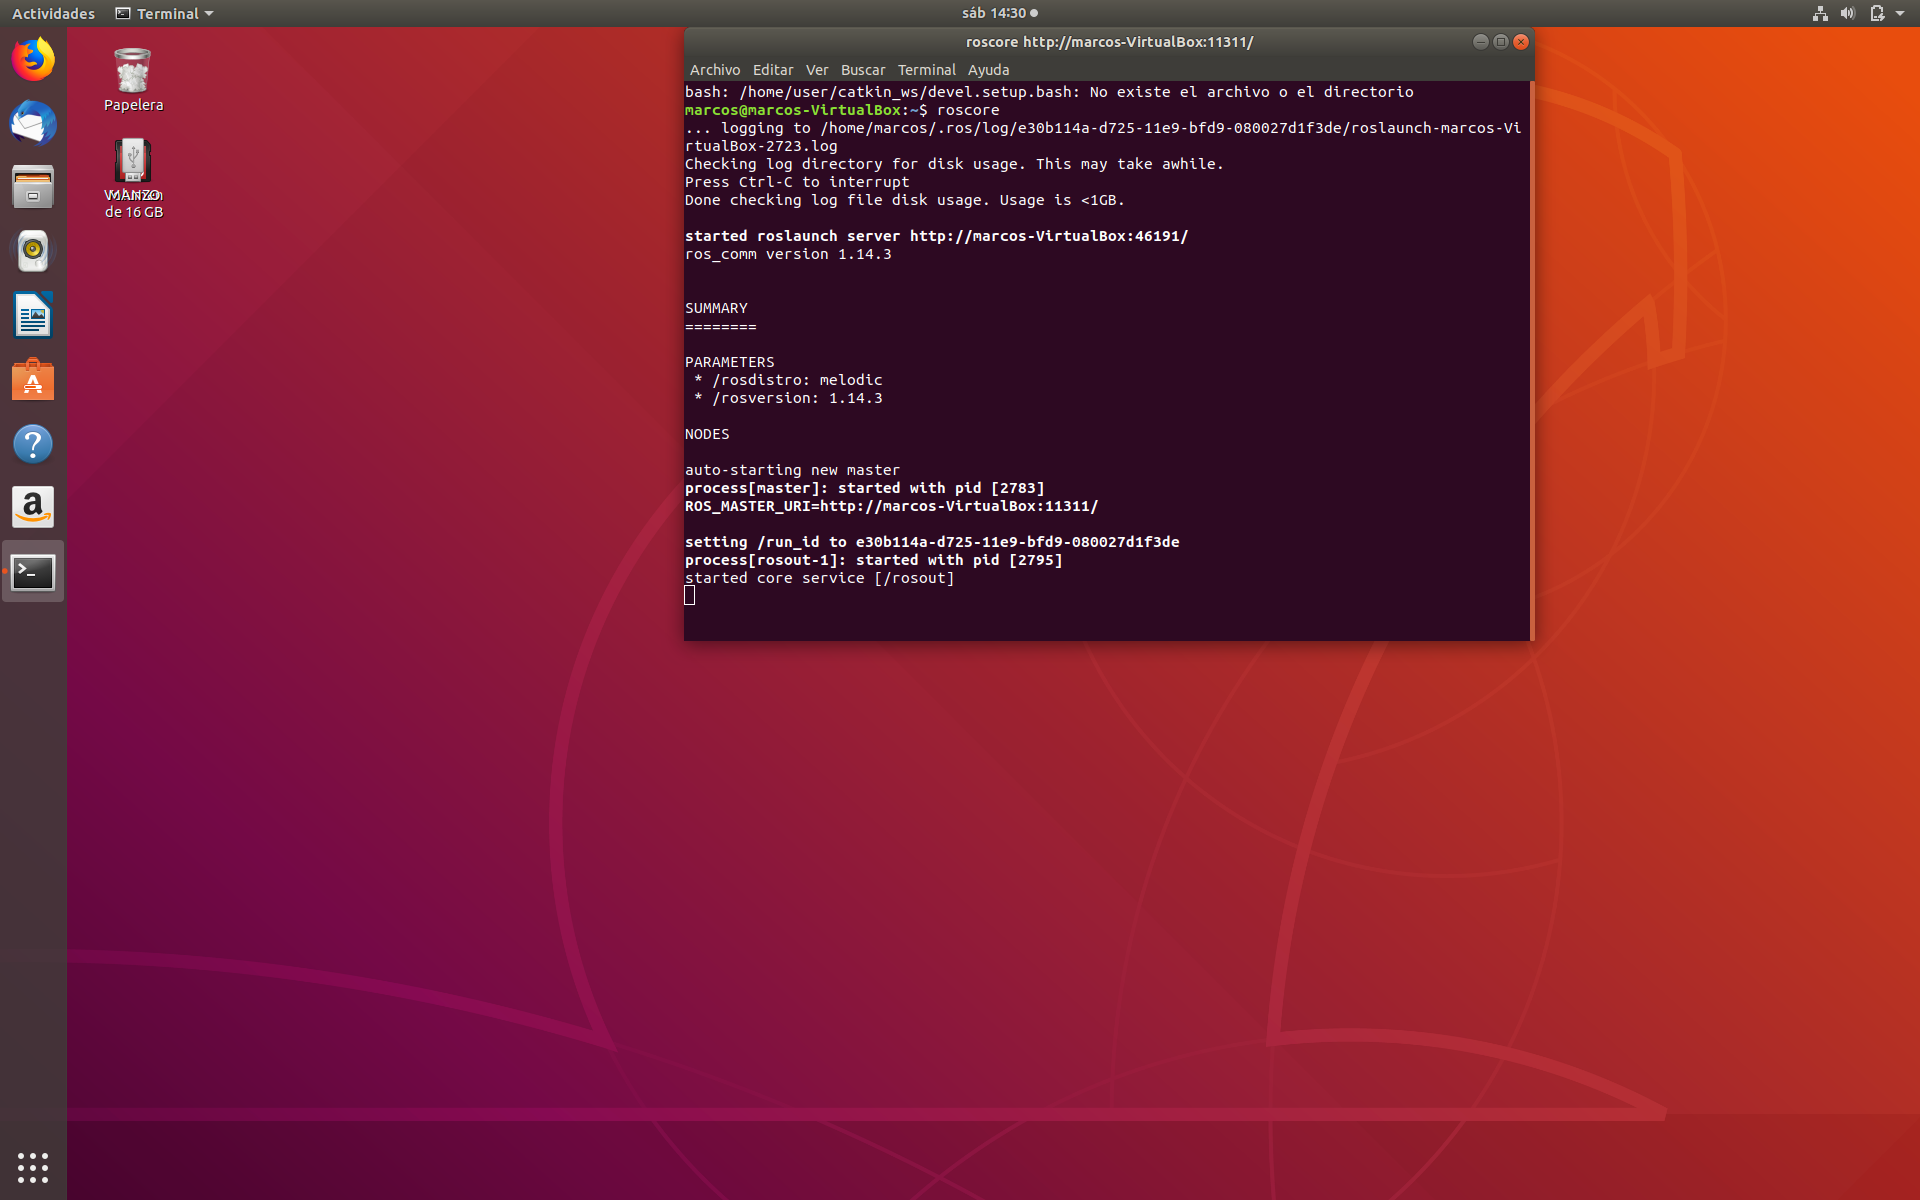
\includegraphics[scale=.15]{link21.png}
\end{figure}
\begin{figure}[h]
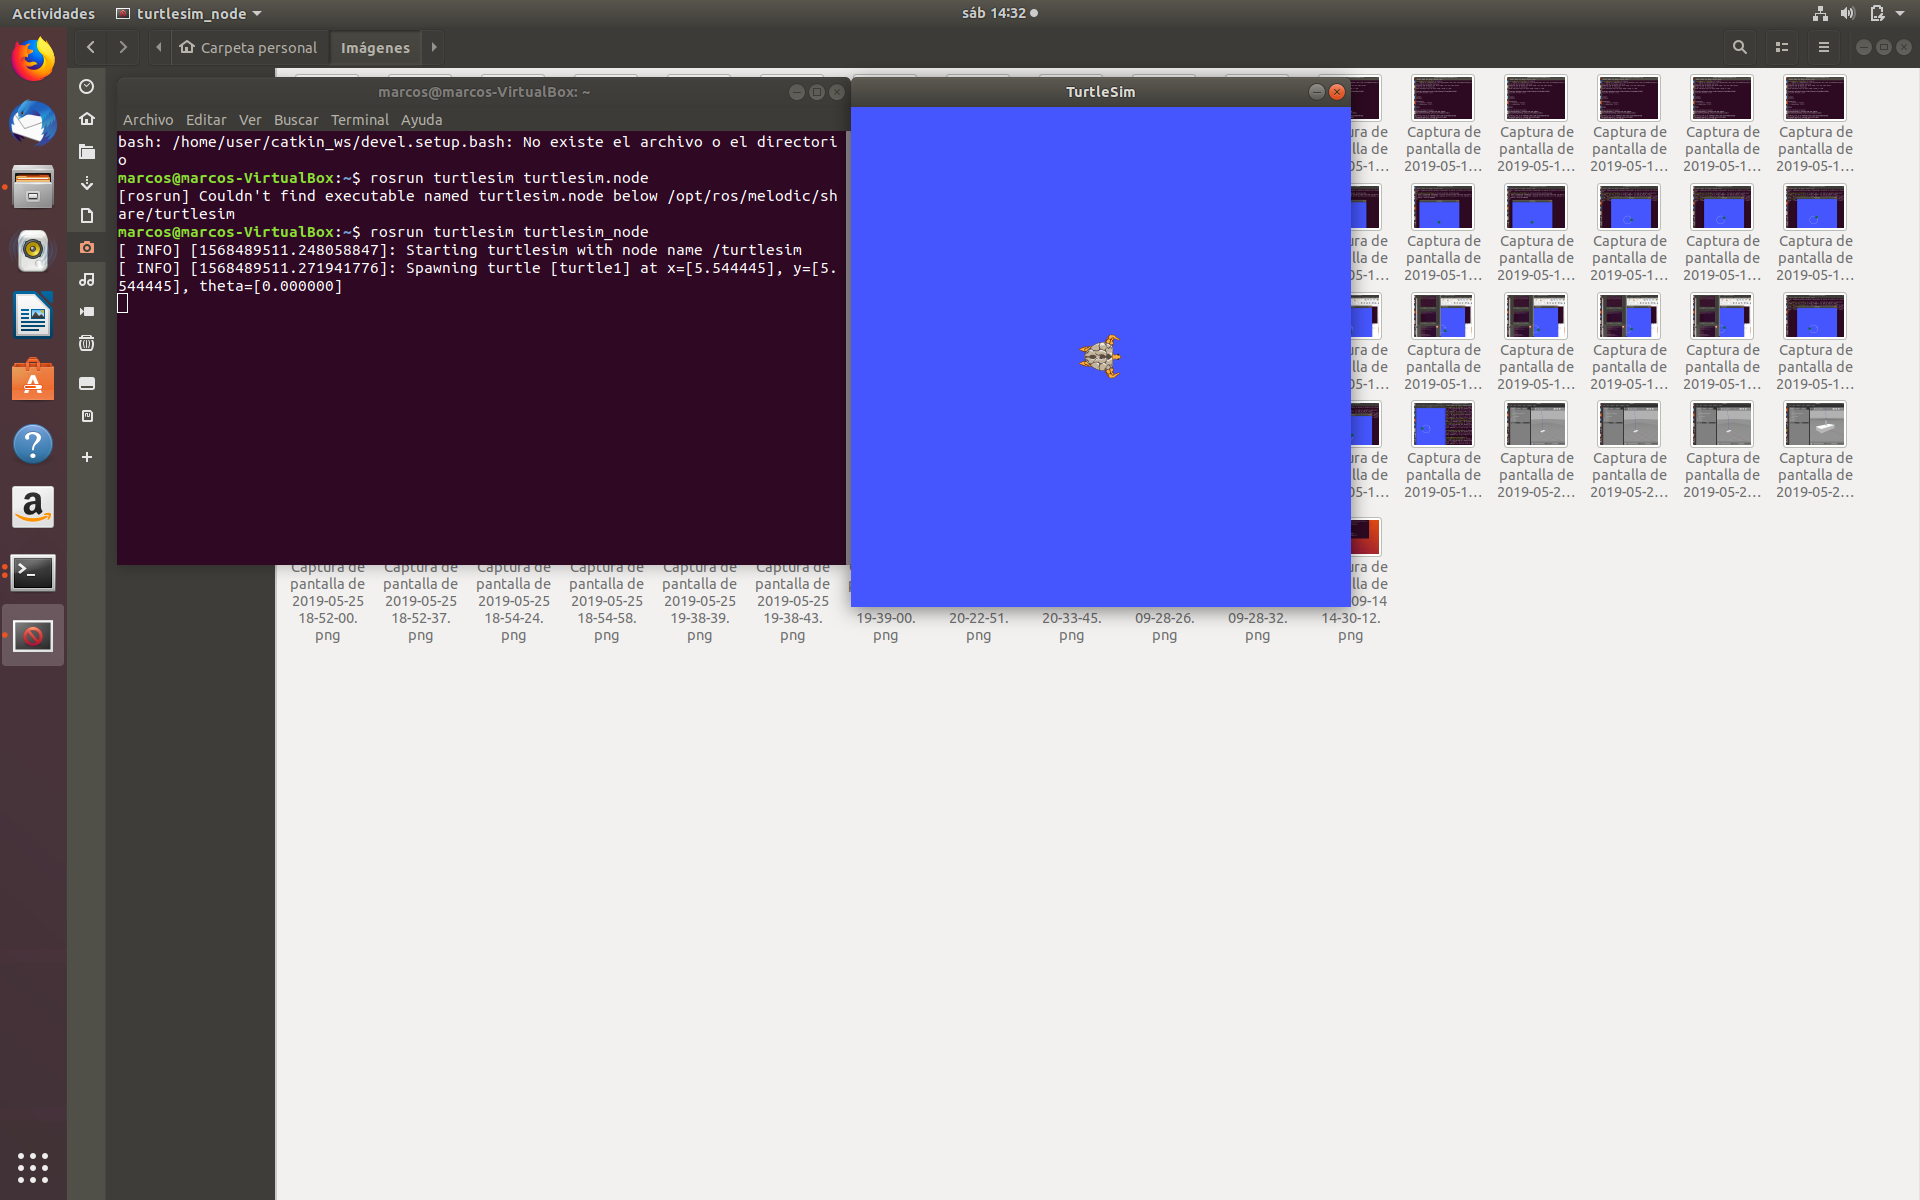
\includegraphics[scale=.15]{link23.png}
\end{figure}

\bibliographystyle{unsrt}
\bibliography{biblio.bib}

\end{document}

